\documentclass{article}

\usepackage[a4paper, total={15cm, 25cm}]{geometry}
\usepackage[utf8]{inputenc}
\usepackage[italian]{babel}

\usepackage{amsmath}
\usepackage{amsthm}
\usepackage{hyperref} 
\usepackage{graphicx}

\theoremstyle{remark}
\newtheorem*{remark}{Osservazione} 

\title{Ottica Fisica}
\author{}
\date{}

\begin{document}
\maketitle

\subsection*{Equazione di Helmholtz}
Dalle equazioni di Maxwell per un mezzo dielettrico omogeneo si ottiene la relazione:
\begin{equation} \label{eq:equazione_onde_mezzo}
c^2\nabla^2 \overrightarrow{E} = \frac{\partial^2 E}{\partial t^2} + \frac{1}{\varepsilon_0} \frac{\partial^2 \overrightarrow{P}(\overrightarrow{E})}{\partial t^2}
\end{equation}
Per mezzi lineari, tra $E$ e $P$ si ha la seguente relazione:
\begin{equation*}
\overrightarrow{P} = \varepsilon_0 \chi \overrightarrow{E}
\end{equation*}
Passiamo ora nel dominio delle frequenze per semplificare le operazioni di derivazione nella \eqref{eq:equazione_onde_mezzo} per ottenere l'equazione di Helmholtz:
\begin{equation}	\label{eq:equazione_helmholtz}
\nabla^2 \overrightarrow{\tilde{E}}(\overrightarrow{r}) + \left(\frac{\omega}{c}\right)^2 \frac{\varepsilon(\omega)}{\varepsilon_0} \overrightarrow{\tilde{E}}(\overrightarrow{r}) = 0
\end{equation}
Questa equazione impone una condizione sulla parte spaziale del campo elettrico. La parte temporale è contenuta all'interno del termine $\epsilon(\omega)$ per mezzi omogenei e lineari.\\
\\
La forma generale dell'equazione di Helmholtz è la seguente:
\begin{equation} 	\label{eq:equzione_generale_helmholtz}
\nabla^2 F + k^2 F = 0
\end{equation}
con $k$ vettore d'onda.\\
\\
Quindi dalla \eqref{eq:equazione_helmholtz} e dalla \eqref{eq:equzione_generale_helmholtz} si ha la relazione:
\begin{equation*}
k = \frac{\omega}{c} \sqrt{\frac{\varepsilon(\omega)}{\varepsilon_0}}
\end{equation*}
chiamata anche relazione di dispersione.\\
\\
\\
In conclusione, passando all'equazione di Helmholtz si ricavano ulteriori informazioni riguardo le onde, ma si perde la relazione tra campo elettrico e campo magnetico. Siccome le onde devono sottostare anche alle equazioni di Maxwell, è sufficiente reintrodurre $B$ di modo da ottenere che:
\begin{equation*}
\overrightarrow{B} = \frac{1}{\omega} \overrightarrow{k} \times \overrightarrow{E}
\end{equation*}

\vfill
\hrule
\subsubsection*{Extra:}
\href{https://physics.stackexchange.com/questions/334084/wave-vs-helmholtz-equation}{More on Helmholtz's equation...}

\newpage

\section*{Ottica Geometrica}
In questa sezione si cercherà di descrivere la propagazione delle onde elettromagnetiche in condizioni più complesse come superfici curve, dielettrici non omogenei etc.
Per evitare di dover risolvere l'equazione di Helmholtz tutte le volte che ci si presenta un problema di questo fare un'approssimazione che caratterizza l'ottica geometrica.
Ipotizziamo che:
\begin{equation*}
k_0 \rightarrow \infty \qquad \lambda_0 \rightarrow 0
\end{equation*}
\subsubsection*{Principio di Fermat}
La luce percorre una traiettoria chiamata raggio. Essa è la traiettoria con il minor tempo di percorrenza, quindi non necessariamente quello più breve; in particolare quando la luce attraversa dielettrici con $n$ diversi viaggia una distanza minore nel dielettrico più lento ottimizzando il tempo di volo.\\
Legge di trasformazione dei raggi:
\begin{equation}	\label{eq:legge_di_trasf_dei_raggi}
n_1 \sin\theta_i - n_2 \sin\theta_t = 0
\end{equation}
La quale è simile alla legge di Snell ma, per come è stata ricavata, la \eqref{eq:legge_di_trasf_dei_raggi} non si limita ad un'onda incidente su una superficie piatta ma include qualsiasi geometria dell'interfaccia.

\subsubsection*{Immagine reale e immagine virtuale}
Si ha un'immagine reale quando i raggi che giungono al sensore provengono da un punto che coincide con la posizione dell'oggetto stesso. Nel caso in cui il punto dove convergono i raggi non sia quello dove l'oggetto è posizionato allora si parla di immagine virtuale.

\subsection*{Superfici cartesiane}
$\cdots$

\subsection*{Regime parassiale}
Il regime parassiale consiste nel considerare solo raggi incidenti il sistema ottico con angoli molto piccoli rispetto all'asse di quest'ultimo.\\
Con questa approssimazione possiamo associare una relazione lineare tra la posizione e l'angolo di entrata e uscita del raggio nel e dal sistema ottico.\\
Questa relazione è scrivibile sotto forma di matrice del tipo:
\[
\begin{bmatrix}
y_1\\
\alpha_1
\end{bmatrix}
=
\begin{bmatrix}
A	&	B\\
C	&	D
\end{bmatrix}
\begin{bmatrix}
y_0\\
\alpha_0
\end{bmatrix}
\]

\subsubsection*{Matrice di propagazione libera}
Nel caso in cui il sistema ottico non contenga nessun elemento ottico, allora si ha una propagazione libera del raggio su un percorso $L$.
\[
\begin{bmatrix}
y_1\\
\alpha_1
\end{bmatrix}
=
\begin{bmatrix}
1	&	L\\
0	&	1
\end{bmatrix}
\begin{bmatrix}
y_0\\
\alpha_0
\end{bmatrix}
\]

\subsubsection*{Matrice per superfici sferiche}
\[
\begin{bmatrix}
y_1\\
\alpha_1
\end{bmatrix}
=
\begin{bmatrix}
1	&	0\\
\frac{1}{R}(\frac{n}{n'}-1)	&	\frac{n}{n'}
\end{bmatrix}
\begin{bmatrix}
y_0\\
\alpha_0
\end{bmatrix}
\]
Questa relazione vale per qualsiasi superficie sferica di raggio $R$ sia essa concava o convessa. Se la superficie è convessa (se C si trova a destra del vertice V) R è assunto positivo altrimenti negativo.

\subsubsection*{Generalizzazione dei sistemi ottici}
Il concetto di sistema ottico è stato introdotto per semplificare l'analisi di sistemi con elementi ottici numerosi. Associando ad ogni elemento ottico la sua matrice $M_i$ è possibile ricavare la matrice di trasferimento $M$ totale, detta anche diottro sferico, che relaziona entrata e uscita dei raggi da tutti i sistemi ottici come se fosse uno solo.
\[
\begin{bmatrix}
y_N\\
\alpha_N
\end{bmatrix}
=
M_N M_{N-1} \cdots M_2 M_1
\begin{bmatrix}
y_0\\
\alpha_0
\end{bmatrix}
\]
Osservazione:
Da notare che la moltiplicazione delle matrici segue il verso opposto (da destra a sinistra) del percorso del raggio (da sinistra a destra).\\
Osservazione:
Durante la risoluzione degli esercizi può essere opportuno verificare il calcolo della matrice $M$ calcolandone il determinante. Infatti deve essere:
\begin{equation*}
\det M = \frac{n_0}{n_f}
\end{equation*}
Con $n_0$ indice di rifrazione del mezzo da cui parte il raggio e $n_f$ indice di rifrazione del mezzo in cui arriva il raggio.

\subsubsection*{Proprietà della matrice di trasferimento}
\begin{itemize}
\item $D = 0$
\end{itemize}
\begin{minipage}{.5\textwidth}
\[
\begin{cases}
y_f = Ay_0 + B\alpha_0\\
\alpha_f = Cy_0
\end{cases}
\]
\end{minipage}
\begin{minipage}{.5\textwidth}
	\centering
    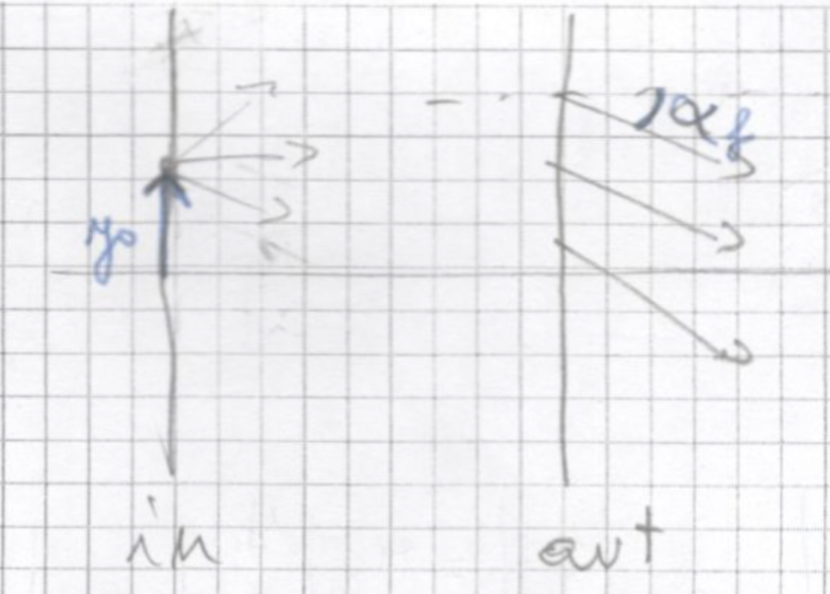
\includegraphics[height=4cm]{images/d_nullo}
\end{minipage}
I raggi finali avranno altezza diversa ma l'angolo con cui escono è lo stesso (raggi paralleli tra loro).
\begin{itemize}
\item $A = 0$
\end{itemize}
\begin{minipage}{.5\textwidth}
\[
\begin{cases}
y_f = B\alpha_0\\
\alpha_f = Cy_0 + D\alpha_0
\end{cases}
\]
\end{minipage}
\begin{minipage}{.5\textwidth}
	\centering
    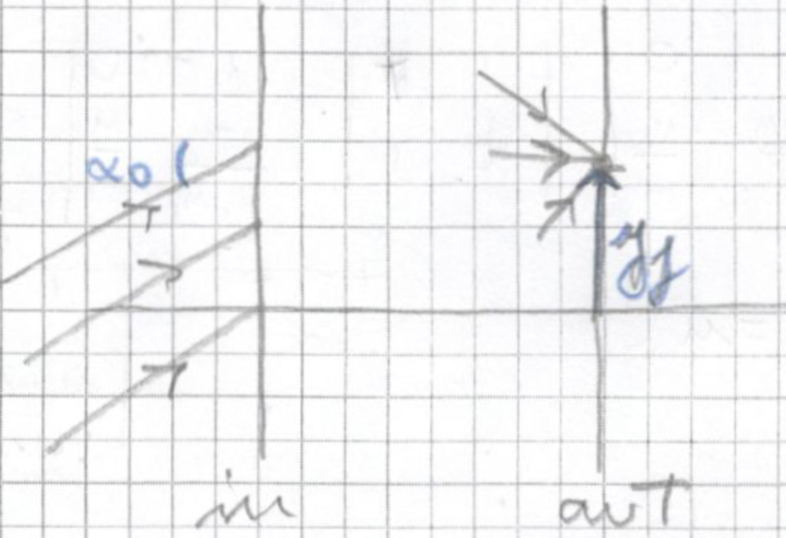
\includegraphics[height=4cm]{images/a_nullo}
\end{minipage}
In ingresso si hanno raggi con stesso angolo $\alpha_0$ (paralleli) ma diversa altezza $y_0$.\\
In uscita li trovo tutti nello stesso punto ad altezza $y_f$.
\begin{itemize}
\item $B = 0$
\end{itemize}
\begin{minipage}{.5\textwidth}
\[
\begin{cases}
y_f = Ay_0\\
\alpha_f = Cy_0 + D\alpha_0
\end{cases}
\]
\end{minipage}
\begin{minipage}{.5\textwidth}
	\centering
    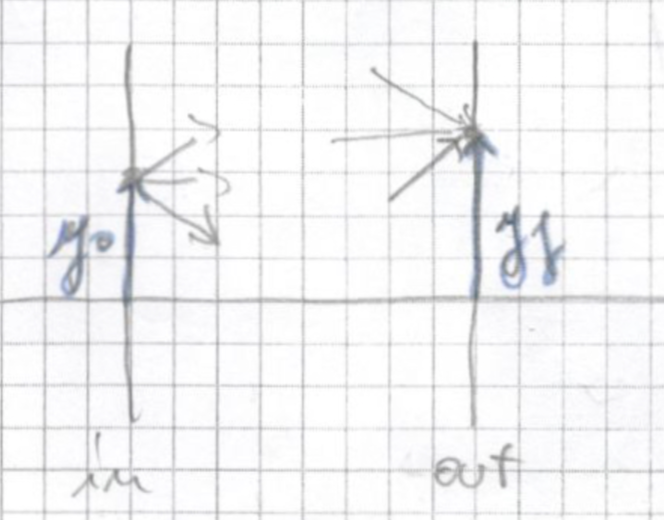
\includegraphics[height=4cm]{images/b_nullo}
\end{minipage}
Tutti i raggi che entrano ad $y_0$ escono ad $y_f$.\\
Ci sono due piani coniugati del sistema ottico: ogni punto ad altezza $y_0$ genera un punto a $y_f$.\\
\centerline{$A = \frac{y_f}{y_0}$ \qquad ingrandimento del sistema ottico}
\begin{itemize}
\item $C = 0$
\end{itemize}
\begin{minipage}{.5\textwidth}
\[
\begin{cases}
y_f = Ay_0 + B\alpha_0\\
\alpha_f = D\alpha_0
\end{cases}
\]
\end{minipage}
\begin{minipage}{.5\textwidth}
	\centering
    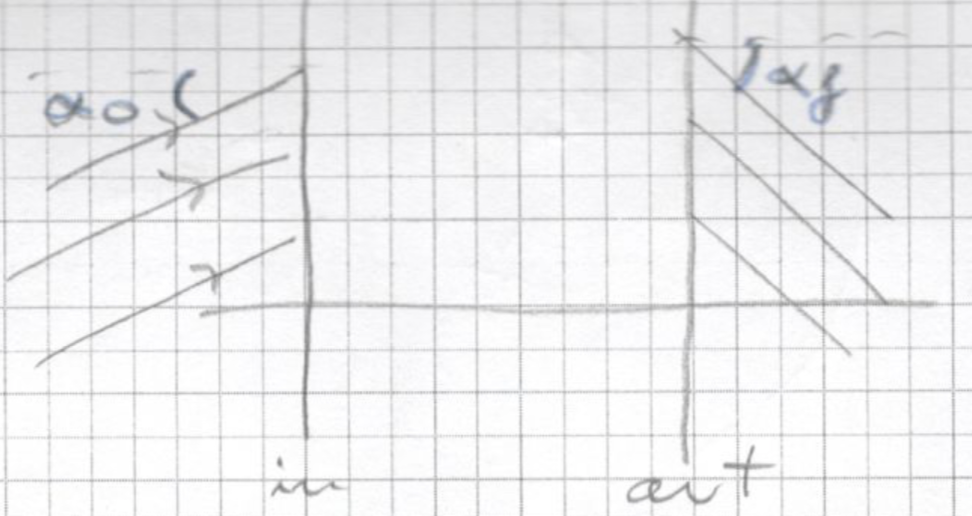
\includegraphics[height=4cm]{images/c_nullo}
\end{minipage}
Tutti i raggi paralleli in entrata avranno raggi paralleli anche in uscita.\\
\centerline{$D = \frac{\alpha_f}{\alpha_0}$	\qquad ingrandimento angolare}

\subsection*{Punti cardinali}
Per un qualsiasi sistema ottico è possibile fare un'analisi riducendolo ad una semplice lente spessa o diottro. Per fare ciò definiamo dei punti cardinali che utilizzeremo per effettuare la suddetta analisi.\\
\begin{figure}[h]
\centering
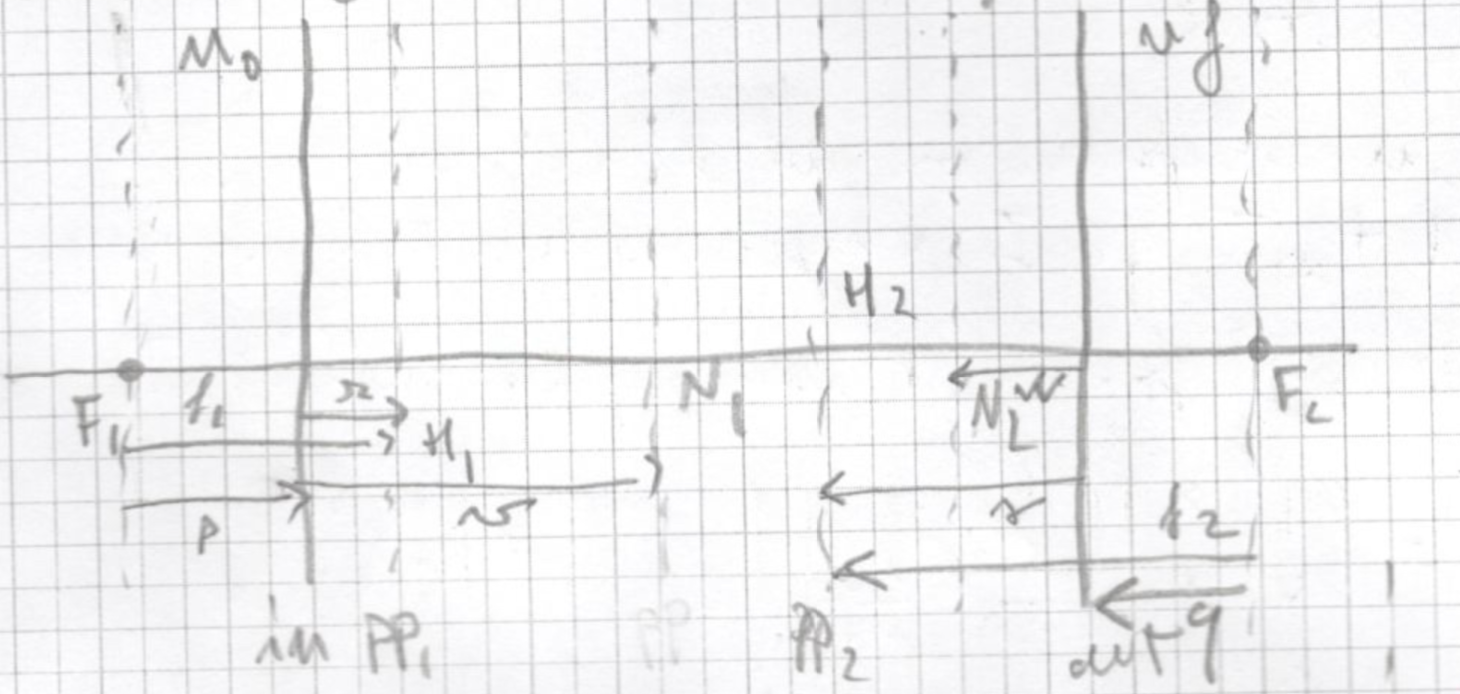
\includegraphics[height=4cm]{images/lente_spessa}
\end{figure}
\\
Distanza tra il piano focale $F_1$ e il piano principale $PP_1$:
\begin{equation*}
p = \frac{D}{C}
\end{equation*}
Distanza tra il piano ($IN$) di entrata, che corrisponde con la superficie della lente, e il piano principale ($PP_1$):
\begin{equation*}
r = p - f_1 = \frac{D}{C} - \frac{n_0}{n_f} \frac{1}{C} = \frac{1}{C} \left(D - \frac{n_0}{n_f} \right)
\end{equation*}
Distanza del punto nodale $N_1$ da $PP_1$:
\begin{equation*}
v = \frac{D-1}{C}
\end{equation*}
\\
Analogamente si calcolano anche le distanze in uscita.\\
Distanza tra il piano focale $F_2$ e il piano principale $PP_2$:
\begin{equation*}
q = - \frac{A}{C}
\end{equation*}
Distanza tra il piano ($OUT$) di uscito, che corrisponde con l'altra superficie della lente, e il piano principale ($PP_2$)
\begin{equation*}
s = \frac{1-A}{C}
\end{equation*}
Distanza del punto nodale $N_2$ da $PP_2$:
\begin{equation*}
w = \frac{-A}{C}
\end{equation*}
\begin{remark}
nel caso in cui $n_0 = n_f$ si ha che:
\begin{equation*}
f_2 = - \frac{1}{C} = - f_1 \qquad \|f_1\| = f_2
\end{equation*}
\begin{equation*}
r = v \qquad s = w
\end{equation*}
Inoltre coincidono i punti principali (intersezione tra piani principali PP e asse ottico) e i punti normali.
\begin{equation*}
H_1 \equiv N_1 \qquad H_2 \equiv N_2
\end{equation*}
\end{remark}
In conclusione, conoscendo la matrice di trasferimento è possibile ricavare tutte le distanze e i punti cardinali.
\newpage

\section*{Ottica Diffrattiva}
\end{document}
